\documentclass[a4paper,11pt]{article}
%----------------------------------------------------------------------------------------
% Use Package's
%----------------------------------------------------------------------------------------

\usepackage[utf8]{inputenc}
\usepackage{amssymb}
\usepackage{amsmath}
\usepackage{amsthm}
\usepackage{pifont}
\usepackage{mathrsfs}
\usepackage{thmbox} %Leftbar command
\usepackage{fancyhdr} % Required for custom headers
\usepackage{lastpage} % Required to determine the last page for the footer
\usepackage{extramarks} % Required for headers and footers
\usepackage{graphicx} % Required to insert images
\usepackage{lipsum} % Used for inserting dummy ''Lorem ipsum'' text into the template
\usepackage{siunitx}
\usepackage{eurosym}
\usepackage{booktabs}
\usepackage{multicol}
\usepackage{float}
\usepackage{wrapfig}
\usepackage{mathtools}
\usepackage{asymptote}
\usepackage{enumitem} % Custom enumerate for e.g. Ring properties
\usepackage{tikz} % Function diagrams
\usepackage{geometry} % Changing textwidth
% - Code listing with color settings - 
\usepackage{listings}
\usepackage{color}
%\usepackage{pdfpages}
\usepackage{todonotes}
% ----------------- biblatex ----------------- 
\usepackage[backend=biber,sorting=ynt]{biblatex}  %,style=alphabetic
\addbibresource{ref.bib}
% -------------------------------------------- 
\input{lstunputSettings.tex}


\setcounter{MaxMatrixCols}{20}

%----------------------------------------------------------------------------------------
% Page Layout
%----------------------------------------------------------------------------------------
% Margins
\topmargin=-0.4in
\evensidemargin=0in
\oddsidemargin=0in
\textwidth=6.5in
\textheight=9.7in
\headsep=0.25in 

\linespread{1.1} % Line spacing
\setlength{\parskip}{0.5\baselineskip}

% Set up the header and footer (report)
\fancypagestyle{plain}{%first page of chapters
	\fancyhf{}
	\fancyfoot[LO,RE]{\textsc{Jeroen Lammers}}
	\fancyfoot[RO,LE]{\thepage/\pageref{LastPage}}
	\renewcommand{\headrulewidth}{0pt}
	\renewcommand{\footrulewidth}{0.4pt}
}
\pagestyle{fancy} %otherpages
\fancyhf{}% it clears the header and footer, otherwise the elements of the default "plain" page style will appear
\fancyhead[LO,RE]{} 
\fancyhead[CO,CE]{BSc Project}
\fancyhead[RO,LE]{}
\fancyfoot[LO,RE]{}
\fancyfoot[CO,CE]{Jeroen Lammers}
\fancyfoot[RO,LE]{\thepage/\pageref{LastPage}}
\renewcommand\headrulewidth{0.4pt} % Size of the header rule
\renewcommand\footrulewidth{0.4pt} % Size of the footer rule
\setlength{\parindent}{0ex}
%----------------------------------------------------------------------------------------
% New commands
%----------------------------------------------------------------------------------------
\newcommand{\ap}[2]{\underline{\textbf{AP - #1 :}} #2}
\newcommand{\Question}[3]{\large\textbf{#1 (#2) - \normalsize#3} \vspace{15px} }
\newcommand{\Answer}[1]{\begin{tabular}{l p{.9\textwidth} l} \hspace{.05\textwidth}& #1 &\hspace{.05\textwidth} \end{tabular}}

\newcommand{\C}{\mathbb{C}}
\newcommand{\N}{\mathbb{N}}
\newcommand{\R}{\mathbb{R}}

\newcommand{\Def}[2]{\textbf{\large Def: \normalsize#1}\newline \textit{#2}}
\newcommand{\Thr}[2]{\textbf{\large Thr: \normalsize#1}\newline \textit{#2}}
\newcommand{\Lemma}[2]{\textbf{\large Lem: \normalsize#1}\newline \textit{#2}}
\newcommand{\Prop}[2]{\textbf{\large Prop: \normalsize#1}\newline \textit{#2}}
\newcommand{\Cor}[2]{\textbf{\large Cor: \normalsize#1}\newline \textit{#2}}
\newcommand{\claim}[2]{\textbf{\large Claim: \normalsize#1}\newline \Answer{#2}}
\newcommand{\Example}[2]{\textbf{\large Ex: \normalsize#1}\newline \Answer{#2}}
\newcommand{\Proof}[2]{}%\textbf{Proof: #1}\newline \Answer{#2}}
\newcommand{\Note}[2]{\textbf{\large Note: \normalsize#1}\newline #2}
\newcommand{\Remark}[2]{\textbf{\large Remark: \normalsize#1}\newline #2}
\newcommand{\Ex}[3]{\textbf{\large Exercise: \normalsize#1}\newline #2 \newline \newline \Answer{#3}}
%----------------------------------------------------------------------------------------
% Document
%----------------------------------------------------------------------------------------
\begin{document}
% ----------------------------- Abstract ---------------------------- 
%\setcounter{page}{0}
%\includepdf{frontpage.pdf}
%\newpage

% belangrijkste gedeelte
% geeft weer waar het over gaat en resultaten
%\section{Abstract}
In this thesis we deal with implementing the existing data informativity framework into a Matlab toolbox. The toolbox has support for both noiseless data as well as data with bounded noise. In the case of noiseless data there are implementations for system identification, stabilisability, controllability, stability, state feedback, deadbeat control, LQR control, dynamic measurement feedback and state identification. In the case of data with bounded noise there are implementations for quadratic stabilisation, $\mathcal{H}_2$ control and $\mathcal{H}_\infty$ control.
% ----------------------------- Introduction  -----------------------
% meer overcoupelende context
% introduceer onderwerp

\section{Introduction}
% - Context - 
When studying systems and control theory we often focus on finding properties of a given mathematical model. However, in the real world the mathematical model of a system is not always available. In most cases we only have the measurements/data as produced by a system. To combat this, we can use tools from the field of data-driven analysis and control. These tools are able to infer system theoretical properties and stabilising controllers from the data without explicitly knowing the underlying mathematical model of the system.

Since we only have access to the data, we cannot necessarily determine the model that describes this data uniquely. 
It might be the case that there are an infinite amount of different mathematical models describing the same data.
Because of this we will be considering the informativity framework as defined in \cite{waarde2019data} and \cite{waarde2020noisy} which loosely states that if a property holds for all systems describing the data, then the data is informative for that property.

% Problem
% - System & control Matlab use
When applying methods from systems and control to an actual problem, computers are often needed due to the complexity and size of the systems and data. Thus, in this thesis we will implement a Matlab toolbox based on the necessary and sufficient conditions of data informativity from papers, \cite{waarde2019data} and \cite{waarde2020noisy}. 

We will consider exact ( noise free) data and noisy data cases separately. For the latter we consider methods to check if a system is identifiable, controllable, stabilisable or stable. We will also look at how we can construct a stabilising state feedback controller, deadbeat controller, LQR controller and a stabilising dynamic measurement controller directly from the data. In the case of dynamic measurement feedback we will also consider state identification for cases in which we only have access to the input and output data of a system.

% - implementation noisy data
For the case of noisy data we will only look at constructing controller directly from the data, more specifically, we will study how to compute a quadratic stabilising controller, a controller for the $\mathcal{H}_2$ control problem and a controller for the $\mathcal{H}_\infty$ control problem.\newpage
% ----------------------------- Discussion --------------------------
\section{Definitions}
% Abstract of the section
In this section we will introduce the notion of informativity. We will also introduce ourselves with the notation that will be used in the paper to indicate data and systems. 

\subsection{Informativity}
% Introducing the set of systems data informativity
Let $\Sigma$ be the set of discrete time models with a given state space dimension $n$ and a given input space dimension $m$. Then if we have state/input data $\mathcal{D}$ of this form, then we know that the system $\mathcal{S}$ that produced this data is contained in the set $\Sigma$. However, using $\Sigma$ is not very useful unless we reduce the set to be more manageable, we can do this by using our knowledge of the true system, namely the data. We will only consider systems that are able to produce the data, we will call this set $\Sigma_\mathcal{D} \subseteq \Sigma$. 

Suppose we want to show if the true system is controllable, we might not be able to uniquely identify the true system using the data, i.e. $\# \Sigma_\mathcal{D} > 1$. However if we are able to show that every system in the set $\Sigma_\mathcal{D}$ is controllable, then we would also know that the true system is controllable. This is the idea behind data informativity. We say the data $\mathcal{D}$ is informative for a property $\mathcal{P}$ if all systems that describe the data $\Sigma_\mathcal{D}$ have the property $\mathcal{P}$. Let $\Sigma_\mathcal{P} \subseteq \Sigma$ be the set of all systems that have the property $\mathcal{P}$. Then we can reformulate the definition of data informativity as follows.

\Def{Informativity \cite[Def 1]{waarde2019data}}{
	We say that the data $\mathcal{D}$ is informative for a property $\mathcal{P}$ if $\Sigma_\mathcal{D} \subseteq \Sigma_\mathcal{P}$.
}

Suppose that the data describes only the true system, i.e. $\Sigma_{(U_-,X)} = \{ \mathcal{S} \}$ then we know that if a property $\mathcal{P}$ hold for $\mathcal{S}$ then the data is informative for that property. However, in general, just because $\mathcal{S}$ has a property $\mathcal{P}$ does not immediately imply that the data is informative for $\mathcal{P}$ since the data might describe more then one system. Later on we will see this in an example where the data describes infinity many systems. \todo{add reference to example with no identification and state feedback}

We will also focus on control problems. Suppose we want to see if the property 'is stable in full state feedback with a controller $K$' holds on the data, then we need to know if all systems are stabilisable by state feedback using the controller $K$. For this we will define the set of systems that are stabilised using state feedback for the controller $K$ as follows:
\[ \Sigma_K = \{ (A,B) \, | \, A + B \, K \mbox{ is stable} \} \]
Then we have that the data is informative if $\Sigma_\mathcal{D} \subseteq \Sigma_K$. We will generalise this using the following definition.

\Def{Informativity for control \cite[Def 3]{waarde2019data}}{
	We say that the data $\mathcal{D}$ is informative for a property $\mathcal{P}(\cdot)$ if there exists a controller $\mathcal{K}$ such that $\Sigma_\mathcal{D} \subseteq \Sigma_{\mathcal{P}(\mathcal{K})}$.
}


\subsection{Data}
% Introducing the notation for data
We will use the following example \cite[Ex 2]{waarde2019data} to give a more precise definition of data.


Let $n$ be the dimension of the state space and $m$ be the dimension of the input space. Assume that both are known. Then we know that all systems contained in $\Sigma$ are of the form:
\begin{equation}
	\label{isSystem}
	\mathbf{x}(t+1) = A \mathbf{x}(t) + B \mathbf{u}(t)
\end{equation}
Where $\mathbf{x}(t)$ is the $n$-dimensional state vector and $\mathbf{u}(t)$ is the $m$-dimensional input vector evaluated at time $t$. We will assume our data is generated by the 'true' system, we will denote this system as $(A_s , B_s)$. We will now measure the input and state data on $q$ time intervals $\{0,1,\dots,T_i\}$ where $i \in \{1,2,\dots,q\}$. We denote the data collected on one of these intervals as follows:
\begin{align*}
	U^{i}_{-} &= \left[ \begin{array}{cccc} u^{i}(0) & u^{i}(1) & \dots & u^{i}(T_i - 1) \end{array} \right] \\
	X^{i}     &= \left[ \begin{array}{cccc} x^{i}(0) & x^{i}(1) & \dots & x^{i}(T_i) \end{array} \right]
\end{align*}
We will now 'split' the state data into a 'past' and 'future' segment, these are defined similar to $U^i_-$.
\begin{align*}
	X^{i}_{-} &= \left[ \begin{array}{ccc} x^{i}(0) & \dots & x^{i}(T_i - 1) \end{array} \right] \\
	X^{i}_{+} &= \left[ \begin{array}{ccc} x^{i}(1) & \dots & x^{i}(T_i) \end{array} \right]
\end{align*}
With this representation of our state and input data we have that $X^{i}_{+} = A_s \, X^{i}_{-} + B_s \, U^{i}_{-}$. This holds for all measured intervals $i$ of the true system. We will now combine the data of all intervals to get a more general form.
\begin{align*}
	U_{-} &= \left[ \begin{array}{ccc} U^{1}_{-} & \dots & U^{q}_{-} \end{array} \right] &
	X     &= \left[ \begin{array}{ccc} X^{1} & \dots & X^{q} \end{array} \right] \\
	X_{+} &= \left[ \begin{array}{ccc} X^{1}_{+} & \dots & X^{q}_{+} \end{array} \right] &
	X_{-} &= \left[ \begin{array}{ccc} X^{1}_{-} & \dots & X^{q}_{-} \end{array} \right]
\end{align*}
We will define our data $\mathcal{D} := (U_-, X)$. In this example we have that $\Sigma_\mathcal{D} = \Sigma_{(U_-,X)} = \Sigma_{i/s}$ and is defined by:
\[ \Sigma_{(U_-,X)} = \left\{ (A, B) \, | \, X_{+} = \begin{bmatrix} A & B \end{bmatrix} \begin{bmatrix} X_{-} \\ U_{-} \end{bmatrix} \right\} \]
By construction we know that at least the true system $(A_s,B_s)$ is contained in this set.

We can extend this concept to also include the output of a system. Assume we have a system of the form:
\begin{align}
	\label{isoSystem}
	\mathbf{x}(t+1) &= A \mathbf{x}(t) + B \mathbf{u}(t) \\
	\mathbf{y}(t+1) &= C \mathbf{x}(t) + D \mathbf{u}(t)
\end{align}
Let us define $Y_-$ in the following way:
\begin{align*}
	Y_-^i &= \begin{bmatrix}	y^i(0) & y^i(1)& \dots & y^i(T_i-1); \end{bmatrix}\\
	Y_- &= \begin{bmatrix} Y_-^1 & Y_-^2 & \dots & Y_-^q	\end{bmatrix}
\end{align*}
Then we can define the set of systems that can describe the data as follows:
\begin{equation}
\label{isoSet} 
\Sigma_{(U_-,X, Y_-)} = \left\{ (A, B, C, D) \, | \, 
\begin{bmatrix} X_{+} \\ Y_{-} \end{bmatrix} = 
\begin{bmatrix} A & B \\ C & D \end{bmatrix} 
\begin{bmatrix} X_{-} \\ U_{-} \end{bmatrix} \right\} 
\end{equation}

% Combining both consepts for a more precise defenition
 \newpage
\section{System identification}
% Abstract section
In this section we will see how we can use the data to identify the true system. We will first consider the theory and then we will see how this can be implemented. Lastly we will consider an example that we will solve using the Matlab function based on the previously discussed algorithm.

% What is Systems identification
\Def{Informative for system identification \cite[Def 5]{waarde2019data}}{
	We say that the data is informative for system identification if the data only describes a single system, i.e. $\Sigma_\mathcal{D} = \{(A_s,B_s)\}$.
}

% Mathematics
\subsection{Theory}
Consider systems of the form (\ref{isSystem}) and let $(U_-,X)$ be the data generated by the true system. Assume that we have recorded $T$ data points, i.e. the dimension of $U_-$ is $m \times T$ and the dimension of $X$ is $n \times (T+1)$. Recall that the set of systems described by this data is given by:
\begin{equation}
	\tag{\ref{isSet}} 
	\Sigma_{(U_-,X)} = \left\{ (A, B) \, | \, X_{+} = \begin{bmatrix} A & B \end{bmatrix} \begin{bmatrix} X_{-} \\ U_{-} \end{bmatrix} \right\} 
\end{equation}
where $\begin{bmatrix} X_{-} \\ U_{-} \end{bmatrix}$ is $(n+m) \times T$. Suppose that the $rank \begin{bmatrix} X_{-} \\ U_{-} \end{bmatrix} = n+m$, then there exists a right inverse $\begin{bmatrix} V_1 & V_2 \end{bmatrix}$ such that $\begin{bmatrix} X_{-} \\ U_{-} \end{bmatrix} \begin{bmatrix} V_1 & V_2 \end{bmatrix} = I_{n+m}$. If we multiply the equation from (\ref{isSet}) with this inverse we get the following:
\begin{equation*}
	X_{+} \begin{bmatrix} V_1 & V_2 \end{bmatrix} = \begin{bmatrix} A & B \end{bmatrix} I_{n+m}
\end{equation*}
Thus if the data is full rank we are able to retrieve the $(A,B)$ pair directly. This results in the following proposition.

% Pseudo code / algorithm
\subsection{Algorithm}
\Prop{\cite[Prop 6]{waarde2019data}}{
	The data $(U_-,X)$ is informative for system identification if and only if:
	\begin{equation} \label{SysIdentRankCond}
		rank \begin{bmatrix} X_{-} \\ U_{-} \end{bmatrix} = n+m 
	\end{equation}
	Furthermore, if (\ref{SysIdentRankCond}) holds, then there exists a right inverse $\begin{bmatrix} V_1 & V_2 \end{bmatrix}$ (as defined above), and for any such right inverse $A_s = X_+ V_1$ and $B_s = X_+ V_2$.
}

Suppose we consider a system without any inputs, then the proposition reduces to checking if $X_-$ has full row rank and finding a right inverse $X_-^\dagger$ of $X_-$. Then we retrieve the system as follows $A_s = X_+ X_-^\dagger$.

let us assume we consider an input, state, output system of the form (\ref{isoSystem}). Recall the set of systems described by the data is given by (\ref{isoSet}):
\begin{equation*} \tag{\ref{isoSet}}
\Sigma_{(U_-,X, Y_-)} = \left\{ (A, B, C, D) \, | \, 
\begin{bmatrix} X_{+} \\ Y_{-} \end{bmatrix} = 
\begin{bmatrix} A & B \\ C & D \end{bmatrix} 
\begin{bmatrix} X_{-} \\ U_{-} \end{bmatrix} \right\} 
\end{equation*}
In this case if the proposition holds, we can also retrieve the $C$ and $D$ matrix by computing $C = Y_- V_1$ and $D = Y_- V_2$.

% Example using function
\subsection{Implementation}
\subsubsection*{Syntax}
\mon{[bool, A] = isInformIdentification(X)} \\
\mon{[bool, A, B] = isInformIdentification(X, U)} \\
\mon{[bool, A, B, C, D] = isInformIdentification(X, U, Y)}

\subsubsection*{Description}
\mon{[bool, A] = isInformIdentification(X)}: returns if the state data is informative for system identification, if it is then \mon{A} contains the \mon{A} is the system matrix in state space representation.\\
\mon{[bool, A, B] = isInformIdentification(X, U)}: returns if the state and input data is informative for system identification, if it is then \mon{A} and \mon{B} are the system matrices in state space representation.\\
\mon{[bool, A, B, C, D] = isInformIdentification(X, U, Y)}: returns if the state, input and output data is informative for system identification, if it is then \mon{A}, \mon{B}, \mon{C} and \mon{D} are the system matrices in state space representation.

\subsubsection*{Input arguments}
\textbf{\mon{X}}: State data matrix of dimension $n \times (T+1)$.\\
\textbf{\mon{U}}: Input data matrix of dimension $m \times T$.\\
\textbf{\mon{Y}}: Output data matrix of dimension $p \times T$.

\subsubsection*{Output arguments}
\textbf{\mon{bool}}: (boolean) True if the data is informative for system identification, false otherwise\\
\textbf{\mon{A}}: (matrix) If the data is informative, it contains the systems \mon{A} matrix, empty otherwise.\\
\textbf{\mon{B}}: (matrix) If the data is informative, it contains the systems \mon{B} matrix, empty otherwise.\\
\textbf{\mon{C}}: (matrix) If the data is informative, it contains the systems \mon{C} matrix, empty otherwise.\\
\textbf{\mon{D}}: (matrix) If the data is informative, it contains the systems \mon{D} matrix, empty otherwise.


\subsection{Examples}
Let us consider the following state and input data:
\begin{align*}
	X &= \begin{bmatrix} 0&1&0 \\ 0&0&1 \end{bmatrix} & U = \begin{bmatrix}	1&0	\end{bmatrix}
\end{align*} 
As we can see the data is not sufficient for system identification:
\begin{equation*}
	rank \begin{bmatrix} X_{-} \\ U_{-} \end{bmatrix}  = rank \begin{bmatrix} 0&1 \\ 0&0 \\ 1&0 \end{bmatrix} = 2 \neq 3
\end{equation*}
This is because the data can be generated by systems of the following form:
\[ \Sigma_{i/s} = \left\{ \left( \begin{bmatrix} 0&a_1 \\ 1&a_2 \end{bmatrix}, \begin{bmatrix} 1 \\ 0 \end{bmatrix} \right) \, | \, a_1, a_2 \in \R \right\} \]
However, if we where to consider the same data with 1 additional data point then the data would be informative for system identification:
\begin{align*}
	X_- &= \begin{bmatrix} 0&1&0 \\ 0&0&1 \end{bmatrix} & U &= \begin{bmatrix}	1&0&\alpha	\end{bmatrix} & rank \begin{bmatrix} 0&1&0 \\ 0&0&1 \\ 1&0&\alpha \end{bmatrix} = 3
\end{align*} 
We can also find the same results using the MatLab functions:
\begin{lstlisting}
X = [0 1 0 ; 0 0 1]; U = [1 0];
[bool, A, B] = isInformIdentification(X, U)
\end{lstlisting}
which will return: \mon{[ false, [], [] ]}.




\newpage
\section{Controllability}
% Abstract section
In this section we will see how we can use the data to conclude if a set of systems are controllable of not. We will first consider the mathematics and then we will see how this can be implemented. Lastly we will consider an example that we will solve using the Matlab function based on the previously discussed algorithm.

% What is controllability
\Def{Informative for controllability \cite[Def 7]{waarde2019data}}{
	We say that the data is informative for controllability if all systems that describe the data are controllable. I.e. $\Sigma_{i/o} \subseteq \left\{ (A,B) \, | \, (A,B) \mbox{ is controllable} \right\}$.
}

% Mathematics
We will base our algorithm on theorem 8 and remark 9 from \cite{waarde2019data}. These give necessary and sufficient conditions for the informativity.

\Thr{Informative for controllability}{
	The data $(U_-, X)$ is informative for controllability if and only if $rank(X_+ - \lambda X_- ) = n$ $\forall \lambda \in \mathbb{C}$.
}

This theorem can be reduced to check a finite amount of complex numbers similar to the Hautus test. We have that the above theorem is equivalent to $rank(X+) = n$ and $rank(X_+ - \lambda X_-) = n$ for all $\lambda \neq 0$ with $\lambda^{-1} \in \sigma(X_- X_+^\dagger)$ with $X_+^\dagger$ being the right inverse of $X_+$ and $\sigma(\cdot)$ denotes the set of eigenvalues of the matrix.

% Proof?
%\todo{proof?}

% Pseudo code / algorithm
%This will result in the following pseudo code for the algorithm:
%\begin{lstlisting}
%provide X_ and X+
%if X_ has full row rank
%	for each non zero eigenvalue (lambda) of X_ * X+^-i (X+^-i : right inverse of X+) 
%	check if rank(X+ - \lambda X_) = n
%	if it holds for all eigenvalues then
%		The data is informative for controllability
%else 
%	The data is not informative for controllability
%\end{lstlisting}

% Example using function
\subsection{Implementation}
The algorithm above is implemented in the following functions:
\subsubsection*{Syntax}
\mon{[bool] = isInformControllable(X)} 

\subsubsection*{Description}
\mon{[bool] = isInformControllable(X)}: Returns if the state data from an input-state dataset is informative for controllability.

\subsubsection*{Input arguments}
\textbf{\mon{X}}: State data matrix of dimension $n \times T+1$ from an input-state dataset.

\subsubsection*{Output arguments}
\textbf{\mon{bool}}: (boolean) True if the data is informative for controllability, false otherwise

\subsection{Examples} \label{NotIdentifyButControllable}
We will consider the same data as we did in the example of system identification. Recall the provided data was:
\begin{align*}
X &= \begin{bmatrix} 0&1&0 \\ 0&0&1 \end{bmatrix} & U = \begin{bmatrix}	1&0	\end{bmatrix}
\end{align*} 
For the data to be informative for controllability we need that $X_+ - \lambda X_-$ is full row rank for all $\lambda \in \mathbb{C}$.
\begin{align*}
rank(X_+ - \lambda X_-) = rank\left(\begin{bmatrix} 1&0\\0&1\end{bmatrix} - \begin{bmatrix} 0&\lambda\\0&0\end{bmatrix}\right) = 2
\end{align*}
Hence the data is informative for controllability. 

We can also find the same result by using the Matlab function:
\begin{lstlisting}
X = [0 1 0 ; 0 0 1]; U = [1 0];
[bool] = isInformControllable(X)
\end{lstlisting}
Which will return: \mon{[ 1 ]}.

We can verify the result by considering the systems that generate this data. Recall that the data is generated by systems of the form:
\[ \Sigma_{i/s} = \left\{ \left( \begin{bmatrix} 0&a_1 \\ 1&a_2 \end{bmatrix}, \begin{bmatrix} 1 \\ 0 \end{bmatrix} \right) \, | \, a_1, a_2 \in \R \right\} \]
Thus the controllability matrix is given by:
\[ \begin{bmatrix} B& AB \end{bmatrix} = \begin{bmatrix} 1 & 0 \\ 0 & 1 \end{bmatrix} \]
Since the controllability matrix has full rank we can conclude that systems of this form are indeed controllable.
































\newpage
\section{Stabilisability}
% Abstract section


% What is Stabilisability


% Mathematics


% Proof?


% Pseudo code / algorithm


% Example using function
\subsection{Examples using implementation}
The algorithm above is implemented in the following functions:
\subsubsection*{Syntax}
\mon{[bool] = isInformStabilisable(X)} \\
\mon{[bool] = isInformStabilisable(X, tolerance)}

\subsubsection*{Description}
\mon{[bool] = isInformStabilisable(X)}: Returns if the data is informative for stabilisability. Uses default tolerance of \mon{1e-14}.\\
\mon{[bool] = isInformStabilisable(X, tolerance)}: Returns if the data is informative for stabilisability given a specific tolerance.  

\subsubsection*{Input arguments}
\textbf{\mon{X}}: State data matrix of dimension $n \times T+1$.\\
\textbf{\mon{tolerance}}: Tolerance used for determining when a value is zero up to machine precision. Default value is \mon{1e-14}.

\subsubsection*{Output arguments}
\textbf{\mon{bool}}: (boolean) True if the data is informative for stabilisability, false otherwise\\

\subsubsection{Examples}\newpage
\section{Stability}
% Abstract section


% What is Stability


% Mathematics


% Proof?


% Pseudo code / algorithm


% Example using function
\subsection{Examples using implementation}
The algorithm above is implemented in the following functions:
\subsubsection*{Syntax}
\mon{[bool] = isInformStable(X)}

\subsubsection*{Description}
\mon{[bool] = isInformStable(X)}: Returns if the data of a unforced system is informative for stability.

\subsubsection*{Input arguments}
\textbf{\mon{X}}: State data matrix of dimension $n \times T+1$.

\subsubsection*{Output arguments}
\textbf{\mon{bool}}: (boolean) True if the data is informative for stability, false otherwise

\subsubsection{Examples}\newpage
\section{State feedback}
% Abstract section


% What is State feedback


% Mathematics


% Proof?


% Pseudo code / algorithm


% Example using function
\subsection{Examples using implementation}
The algorithm above is implemented in the following functions:
\subsubsection*{Syntax}
\mon{[bool, K, diagnostics] = isInformStateFeedback(X, U)} \\
\mon{[bool, K, diagnostics] = isInformStateFeedback(X, U, tolerance)} \\
\mon{[bool, K, diagnostics] = isInformStateFeedback(X, U, tolerance, options)}

\subsubsection*{Description}
\mon{[bool, K, diagnostics] = isInformStateFeedback(X, U)}: Returns if the data is informative for stabilisation by state feedback. If so, it also returns a corresponding controller K for closed loop feedback control of the form \mon{A+BK}.\\
\mon{[bool, K, diagnostics] = isInformStateFeedback(X, U, tolerance)}: Returns if the data is informative for stabilisation by state feedback given a specific tolerance. If so, it also returns a corresponding controller K for closed loop feedback control of the form \mon{A+BK}.\\
\mon{[bool, K, diagnostics] = isInformStateFeedback(X, U, tolerance, options)}: Returns if the data is informative for stabilisation by state feedback given a specific tolerance and a spdsettings object. If so, it also returns a corresponding controller K for closed loop feedback control of the form \mon{A+BK}.

\subsubsection*{Input arguments}
\textbf{\mon{X}}: State data matrix of dimension $n \times T+1$.\\
\textbf{\mon{U}}: Input data matrix of dimension $m \times T$.\\
\textbf{\mon{tolerance}}: Tolerance used for determining when a value is zero up to machine precision. Default value is \mon{1e-14}.\\
\textbf{\mon{options}}: sdpsettings used with the Yalmip solver.

\subsubsection*{Output arguments}
\textbf{\mon{bool}}: (boolean) True if the data is informative for stabilisation by state feedback, false otherwise\\
\textbf{\mon{K}}: (matrix) If the data is informative, it contains a stabilising controller \mon{K} for closed loop control \mon{A+BK}, empty otherwise.\\
\textbf{\mon{diagnostics}}: (struct) Diagnostics from the Yalmip \mon{optimize()} function.

\subsubsection{Examples}\newpage
\section{Deadbeat control}
% Abstract section
In this section we will see how we can find a deadbeat controller using only our data. We will first discusse the underlying mathematics after which we will focus on how we can implement this into code. We will also look at a few examples on how to use the provided function.

% What is Deadbeat
\Def{Informative for deadbeat control \cite[Def 20]{waarde2019data}}{
	We say the data $(U_-,X)$ is informative for deadbeat control if there exists a feedback gain $K$ such that $\Sigma_{i/s} \subseteq \Sigma_K^{nil}$. 
}

In other words, the data is informative if we can stabilise all systems described by the data with a given $K$ such that all closed loop systems only have the zero eigenvalue.

% Mathematics
\subsection{Mathematics deadbeat control}
We will begin by considering the following theorem that gives necessary and sufficient conditions for informativity for deadbeat control.

\Thr{\cite[Thr 21]{waarde20}}{
	The data $(U_-,X)$ is informative for deadbeat control if and only if the matrix $X_-$ has full row rank and there exists a right inverse $X_-^\dagger$ of $X_-$ such that $X_+ X_-^\dagger$ is nilpotent. Moreover, if this condition is satisfied then the feedback gain $K := U_- X_-^\dagger$ yields a deadbeat controller.
}

Using this theorem the problem boils down to finding a suitable right inverse such that $X_- X_-^\dagger$ is nilpotent given that $X_-$ has full row rank. We will consider the following 2 cases, first we will look at the case where $X_-$ is a (full rank) square matrix. Second we will look at the case where $X_-$ is a full row rank wide matrix.
 
First lets assume $X_-$ is a square matrix and has full row rank. Then we know that the only right inverse of $X_-$ is its inverse $X_-^{-1}$. Hence the data is informative for deadbeat control if and only if $X_+ X_-^{-1}$ is nilpotent. 

Now lets assume that $X_-$ is a wide matrix and has full row rank. Then there exists an $F \in \R^{T \times n}$ spanning the row space of $X_-$ and an $G \in \R^{T \times (T-n)}$ spanning the null space of $X_-$ such that $\begin{bmatrix}F&G\end{bmatrix}$ is non singular and $X_- \begin{bmatrix}F&G\end{bmatrix} = \begin{bmatrix}I_n&0_{n\times (T-n)}\end{bmatrix}$. Now let $X^\dagger_- = F + G H$ where $H \in \R^{(T-n) \times n}$ if and only if $X_-^\dagger$ is an right inverse of $X_-$.

Proof '$\Rightarrow$': \\
Let $X^\dagger_- = F + G H$ as described above. Then $X_- X^\dagger_- = X_- F + X_- G H = I_n + 0_{n\times (T-n)} * H = I_n$.

Proof '$\Leftarrow$': \\
\todo{add proof}

Thus finding a right inverse such that $X_+ X_-^\dagger$ is nilpotent is equivalent to finding an $H$ such that $X_+ F + X_+ G H$ is nilpotent. Finding this $H$ can be done using pole placement methods for the pair $(X_+ F, X_+ G)$ and placing all eigenvalues at zero.

% Pseudo code / algorithm
\subsection{Algorithm deadbeat control}
Using the mathematics above we can construct an algorithm for checking if the data is informative for deadbeat control and what the corresponding controller is.

\begin{lstlisting}
provide X_, X+ and U
if X_ has full row rank
	if X_ is square
		if X+ * inv(X_) is nilpotent
			The data is informative for deadbeat control
			K = U_ * inv(X_)
	else
		F : spans rowspace of X_ (pseudo inverse of X_ -> pinv(X_)) 
		G : spans the nullspace of X_ (null(X_))
		if (X+ F, X+ G) is controllable
			H = poleplacement(X+ F, X+ G, [0 ... 0])
			The data is informative for deadbeat control
			K = U_ * (F + G H)
The data is not informative for deadbeat control
\end{lstlisting}

However, due to limitation in Matlabs pole placement function we are not able to implement the algorithm into matlab directly. This is because matlab has 2 functions for pole placement, the \mon{place()} function which does not support poles with high multiplicity, which is hence not useable. The other function \mon{acker()} does support pole placement of poles with high multiplicity, but it is limited to a single dimensional input space. Since $X_+ G$ is an $n \times (T-n)$ matrix, we have that our input space is of dimension $T-n$. However, we are able to circumvent this issue by extending the \mon{acker()} function to support higher dinmensional input. To do this we will use the proof of the sufficientcy in theroem 3.29 as well as lemma 3.31 from \cite{bookTrentelman}.

\subsection{Mathematics extending pole placement}

\Lemma{\cite[Lemma 3.31]{bookTrentelman}}{
	If $(A,B)$ is controllable there exist vectors $u_0 , \dots u_{n-1}$ such that the vectors defined by
	\[ x_0 := 0, \, \, \, x_{k+1} := Ax_k + Bu_k \, \, \, (k = 0, \dots , n-1) \]
	are independent.
}

Assume that the pair $(A,B)$ is controllable, we will use \cite[Lemma 3.31]{bookTrentelman} to construct $u_0, \dots , u_{n-1}$ and $x_0,x_1, \dots ,x_n$. We pick $u_n$ to be arbitrary. Then there exists a unique map $F_0$ such that $F_0 x_k = u_k$ for $k = 1,\dots,n$. We can substitute this to get:
\[ x_{k+1} = Ax_k + BF_0 x_k = (A + BF_0 ) x_k \]
for $k \in [1, \dots, n]$. From this we can see that $x_k = (A+BF_0)^{k-1} x_1$. By construction of lemma 3.31 we have that $x_0 = 0$, thus we have $x_1 = A * 0 + B * u_0 = Bu_0$. We will call this $b = Bu_0 = x_1$. By construction $x_1,\dots,x_n$ are independent. Thus we know that the controlability matrix $\begin{bmatrix}b&(A+BF_0)b&\dots&(A+BF_0)^{n-1}b\end{bmatrix} = \begin{bmatrix}x_1&x_2&\dots&x_n\end{bmatrix}$ is full rank. Hence the pair $(A+BF_0,b)$ is controlable. Since the matrix $b$ is a column vector we can use the \mon{acker()} algorithm to compute a suitable controller $f$ such that $A+BF_0 + bf = A + B(F_0 + u_0 f)$ has apropriate eigenvalues. From this we construct the controller $F = F_0 + u_0 f$ that places the eigenvalues in the chosen positions.

\subsection{Algorithm extending pole placement}
We will now rewrite this into pseudo code:
\begin{lstlisting}
Provide A, B and poles
n : dimension of state space
m : dimension of input space
construct linear independent x_1, ... ,x_n from u_0, ..., u_n-1
pick an arbitrary u_n
F0 := [u1 u2 ... un] * inv([x1 x2 ... xn])
b  := B * u0
f  := acker(A + B F0, b, poles)
K  := F0 + u_0 f
\end{lstlisting}

% Example using function
\subsection{Examples using implementation}
The algorithm above is implemented in the following functions:
\subsubsection*{Syntax}
\mon{[bool, K] = isInformDeadbeatControl(X, U)} 

\subsubsection*{Description}
\mon{[bool, K] = isInformDeadbeatControl(X, U)}: Returns if the data is informative for deadbeat control. If so, it also returns a corresponding controller K for closed loop feedback control of the form \mon{A+BK}.

\subsubsection*{Input arguments}
\textbf{\mon{X}}: State data matrix of dimension $n \times T+1$.\\
\textbf{\mon{U}}: Input data matrix of dimension $m \times T$.

\subsubsection*{Output arguments}
\textbf{\mon{bool}}: (boolean) True if the data is informative for deadbeat control, false otherwise\\
\textbf{\mon{K}}: (matrix) If the data is informative, it contains a stabilising controller \mon{K} for closed loop control \mon{A+BK}, empty otherwise.

\subsubsection{Examples}\newpage
\section{Linear quadratic regulation}
% Abstract section
In this section we will see how we can construct a linear quadratic regulator (LQR) based on a given cost function from the input-state data. We will first define what LQR control entails for normal control theory after which we will consider its data-driven dual. We will also see how this data-driven version can be applied to retrieve the controller from the data. Lastly we will see how to solve such a problem both by doing it by hand as well as using the provided Matlab functions.

% What is LQR (normal control)
\subsection{Non data-driven LQR}
We will first revisit the topic of non data-driven LQR. To given an intuitive idea, we want to not only find a solution to the stabilisation problem, we also want to find the best solution given some cost function. Let us consider the discrete-time linear systems of the form $x(t+1) = Ax(t) + Bu(t)$. We will denote the state sequence generated by this system based of a given initial condition $x_0$ and input function $u$ as $x_{x_0 , u}(\cdot)$. We will also define a quadratic cost function associated to the system.
\begin{equation*}
J(x_0 , u) = \sum_{t=0}^{\infty} x^\top (t) Q x (t) + u^\top (t) R u (t)
\end{equation*}
Where $Q$ is symmetric positive semi definite and $R$ is symmetric positive definite. Using this, we want to find for every initial condition $x_0$ an input $\bar{u}$ such that the system stabilises and the cost function is minimised as well as finite, In other words, the $\lim\limits_{t \to \infty} x_{x_0 , \bar{u}}(t) = 0$ given that the cost function $J(x_0 , \bar{u}) \leq J(x_0 , u)$ for all inputs $u$ that cause the system to stabilise. Such an input $\bar{u}$ is called optimal for the given initial condition. As we might expect, an optimal solution does not always exist for every initial condition. Hence we say that an LQR problem is solvable for given $(A,B,Q,R)$ if for every initial condition $x_0$ there exists an optimal solution.

Using the following theorem we can find the solution to the LQR problem. Recall from \cite[Def 3.12]{bookTrentelman} that an eigenvalue is called $(Q,A)$-observable if 
$$rank\begin{pmatrix}A - \lambda I \\ Q \end{pmatrix} = n$$
where $n$ is the dimension of the state space.

\Thr{\cite[Thr 23]{waarde2019data}}
{
	let $Q$ be symmetric positive semi definite and $R$ be symmetric positive definite. Then the following statements hold:
	\begin{enumerate}
		\item If $(A,B)$ is stabilisable, there exists a unique largest real symmetric solution $P^+$ to the discrete-time algebraic Riccati equation
		\begin{equation} \label{DARE}
			P = A^\top P A - A^\top P B (R+B^\top PB)^{-1} B^\top P A + Q
		\end{equation}
		in the sense that $P^+ \geq P$ for every real symmetric $P$ satisfying the discrete-time algebraic Riccati equation. The matrix $P^+$ is positive semi definite.
		\item If, in addition to stabilisability of $(A,B)$, every eigenvalue of $A$ on the unit circle is $(Q,A)$-observable then for every $x_0$ a unique optimal input $\bar{u}$ exists. Furthermore, this input sequence is generated by the feedback law $u = Kx$, where $K$ is given by:
		\begin{equation} \label{LQRK}
			K := -(R+B^\top P^+ B)^{-1} B^\top P^+ A
		\end{equation}
		Moreover, the matrix $A + BK$ is stable.
		\item In fact, the linear quadratic regulator problem is solvable for $(A,B,Q,R)$ if and only if $(A,B)$ is stabilisable and every eigenvalue of $A$ on the unit circle is $(Q,A)$-observable.
	\end{enumerate}
}
If a LQR problem is solvable then we call $K$ the optimal feedback gain for $(A,B,Q,R)$.

% What is LQR (Data driven control)
\subsection{Data-driven LQR}
Now that we have familiarised ourselves with the concept of LQR control we will see how to extend it to data-driven control. We will start by defining the set of systems for which a solution is valid given a feedback gain $K$ and cost matrices $Q$ and $R$.
\[ \Sigma_K^{Q,R} := \left\{ (A,B) \, : \, K \mbox{ is the optimal gain for } (A,B,Q,R) \right\} \]
Using this we can define informativity for linear quadratic regulation as follows.

\Def{Informative for linear quadratic regulation \cite[Def 24]{waarde2019data}}{
	Given matrices $Q$ and $R$, we say that the data $(U_-,X)$ is informative for linear quadratic regulation if there exists feedback gain $K$ such that the optimal gain for all systems is $K$, i.e. $\Sigma_{i/s} \subseteq \Sigma_K^{Q,R}$.
}

We will now consider the following theorem that gives us necessary and sufficient conditions for finding the solution of a data-driven LQR problem.

\Thr{\cite[Thr 26]{waarde2019data}}{
	Let $Q$ be symmetric positive semi definite and $R$ be symmetric positive definite. Then the data $(U_-,X)$ is informative for linear quadratic regulation if and only if at least one of the following two conditions hold:
	\begin{enumerate}
		\item The data $(U_-,X)$ is informative for system identification, that is $\Sigma_{i/s} = \left\{(A_s, B_s)\right\}$, and the linear quadratic regulator problem is solvable for $(A_s,B_s,Q,R)$. In this case, the optimal feedback gain $K$ is of the form (\ref{LQRK}) where $P^+$ is of the form (\ref{DARE}).
		\item For all $(A,B) \in \Sigma_{i/s}$ we have $A = A_s$. Moreover, $A_s$ is stable, $QA_s = 0$, and the optimal feedback gain is given by $K = 0$.
	\end{enumerate}
}

As we can see from the theorem if we are able to identify the system then the data-driven LQR problem reduces to a normal LQR problem for which we have already seen how to solve them. However, there is still the case in which all systems have the same $A = A_s$ matrix, the $A_s$ matrix is inherently stable and $QA_s = 0$. We will now look at why this is a valid solution to the LQR problem in the first place.

Assume we have a $A_s$ which is stable and a $Q$ such that $QA_s = 0$. From this point we assume $B$ to be an arbitrary input matrix of dimension $n \times m$. Since $x(t) \in im(A)$ for all $t > 0$ we have that $Qx(t) = 0$ for all $t>0$ if we pick our input function to be zero. Note that if we pick our input to be zero then the input cost of the cost function will also be zero. Hence the cost will be equal to $J(x_0 , u) = x_0^\top Q x_0$, which is finite. Since the system is inherently stable we know that the system will stabilise without any input. Lastly we note that the cost associated with the initial condition is present in all cost sequences generated for different inputs, hence the zero input case is the minimal solution to the cost function. Hence this case will provide a valid solution to our LQR problem.

However, even though it is a valid solution it is not easily computable in its current form. Hence we will consider the following theorem which rewrites the condition to one of linear matrix inequalities which can be solved by computational means.

\Thr{\cite[Thr 26]{waarde2019data}}{
	Let $Q$ be symmetric positive semi definite and $R$ be symmetric positive definite. Then the data $(U_-,X)$ is informative for linear quadratic regulation if and only if at least one of the following two conditions hold:
	\begin{enumerate}
		\item The data $(U_-,X)$ is informative for system identification, that is $\Sigma_{i/s} = \left\{(A_s, B_s)\right\}$, and the linear quadratic regulator problem is solvable for $(A_s,B_s,Q,R)$. In this case, the optimal feedback gain $K$ is of the form (\ref{LQRK}) where $P^+$ is of the form (\ref{DARE}).
		\item There exists $\Theta \in \mathbb{R}^{T\times n}$ such that $X_-\Theta = (X_-\Theta)^\top$, $U_-\Theta = 0$, $QX_+\Theta=0$ and 
		\[ \begin{bmatrix} X_-\Theta & X_+\Theta \\ \Theta^\top X_+^\top & X_-\Theta \end{bmatrix} > 0 \]
		In this case, the optimal feedback gain $K = 0$.
	\end{enumerate}
}

% Extra notes (optional)


% Example using function
\subsection{Examples using implementation}
The algorithm above is implemented in the following functions:
\subsubsection*{Syntax}
\mon{[bool, K, diagnostics] = isInformLQR(X, U, Q, R)} \\
\mon{[bool, K, diagnostics] = isInformLQR(X, U, Q, R, tolerance)} \\
\mon{[bool, K, diagnostics] = isInformLQR(X, U, Q, R, tolerance, options)}

\subsubsection*{Description}
\mon{[bool, K, diagnostics] = isInformLQR(X, U, Q, R)}: Returns if the data is informative for LQR control. If so, it also returns a corresponding controller \mon{K} for the closed loop feedback control of the form \mon{A+BK}.\\
\mon{[bool, K, diagnostics] = isInformLQR(X, U, Q, R, tolerance)}: Returns if the data is informative for LQR control given a specific tolerance. If so, it also returns a corresponding controller \mon{K} for the closed loop feedback control of the form \mon{A+BK}.\\
\mon{[bool, K, diagnostics] = isInformLQR(X, U, Q, R, tolerance, options)}: Returns if the data is informative for LQR control given a specific tolerance and sdpsettings. If so, it also returns a corresponding controller \mon{K} for the closed loop feedback control of the form \mon{A+BK}.

\subsubsection*{Input arguments}
\textbf{\mon{X}}: State data matrix of dimension $n \times T+1$ from an input-state dataset.\\
\textbf{\mon{U}}: Input data matrix of dimension $m \times T$ from an input-state dataset.\\
\textbf{\mon{Q}}: State cost matrix.\\
\textbf{\mon{R}}: Input cost matrix.\\
\textbf{\mon{tolerance}}: Tolerance used for determining when a value is zero up to machine precision. Default value is \mon{1e-14}.\\
\textbf{\mon{options}}: sdpsettings used with the Yalmip solver.

\subsubsection*{Output arguments}
\textbf{\mon{bool}}: (boolean) True if the data is informative for system identification, false otherwise\\
\textbf{\mon{K}}: (matrix) If the data is informative, it contains a stabilising controller \mon{K} for closed loop control \mon{A+BK}, empty otherwise.\\
\textbf{\mon{diagnostics}}: (struct) Diagnostics from the Yalmip \mon{optimize()} function.


\subsubsection{Examples}
We will consider an example in which all systems have the same $A$ matrix, $A$ is stable and $QA = 0$. We will pick the input data in such a way that it is not full rank. For this we will use the following data
\begin{align*}
X &= \begin{bmatrix} 1&1.5&1.75 \end{bmatrix} & 
U &= \begin{bmatrix} 1&1\\0&0 \end{bmatrix} & 
Q &= \begin{bmatrix} 0 \end{bmatrix} &
R &= \begin{bmatrix} 1&0\\0&1 \end{bmatrix}
\end{align*} 
Note that the choice of $R$ is arbitrary since we have picked the example such that the optimal input will be no input. We will start by checking $U_- \Theta = 0$.
\begin{align*}
U_- \Theta &= 0 \\
\begin{bmatrix} 1&1\\0&0 \end{bmatrix}\begin{bmatrix} a\\b \end{bmatrix} &= \begin{bmatrix} a + b\\0 \end{bmatrix}
\end{align*}
Hence $\Theta = \begin{bmatrix} a & -a \end{bmatrix}^\top$. Since $Q = 0$ we know that $QX_+\Theta = 0$ is satisfied. We also know that $X_-\Theta = (X_-\Theta)^\top$ will hold since $X_-\Theta$ will be a scaler. Hence we only need to check the matrix inequality.
\[ \begin{bmatrix} X_-\Theta & X_+\Theta \\ \Theta^\top X_+^\top & X_-\Theta \end{bmatrix} = 
\begin{bmatrix} \frac{1}{2} a & \frac{1}{4} a \\ \frac{1}{4} a & \frac{1}{2} a \end{bmatrix}
 > 0 \]
If we pick $a = 1$ then the eigenvalues of the matrix will be $\{\frac{1}{4}, \frac{3}{4}\}$ and hence the matrix inequality is satisfied.


We can also find the same result by using the Matlab function:
\begin{lstlisting}
X = [1 1.5 1.75];
U = [1 1 ; 0 0];
Q = [0];
R = [1 0 ; 0 1];
[bool, K] = isInformLQR(X, U, Q, R)
\end{lstlisting}
Which will return: \mon{[ 1, [0 ; 0] ]}.
\newpage
\section{Dynamic measurement feedback}
% Abstract section
In this section we will consider input-state-output systems and how we can use their data to construct a dynamic measurement controller that stabilises the closed loop system. We will start by recalling what a dynamic measurement controller entails. After which we will consider how we can extend this to data-driven control and how we can define the set of systems as well as informativity. We will then consider how we can find necessary and sufficient conditions for finding a dynamic measurement controller for input-state-output data. In the next section we will introduce the consept of state estimation which we will use to extend our theory about dynamic measurement feedback to work using only input and output data.

% Introduce Dynamic feedback control for normal control (reference to Trentelman book)
\subsection{Non-data driven dynamic feedback control}
In this section we will consider discrete time systems that are of the following form.
\begin{subequations}\label{outputSys}
	\begin{align} 
		x(t+1) &= A_s x(t) + B_s u(t) \\
		y(t)   &= C_s x(t) + D_s u(t)
	\end{align}
\end{subequations}

Instead of only using state feedback we will also add an observer to the loop. By combining the observer and the state feedback we get a dynamic measurement controller (see \cite[section 3.12]{bookTrentelman}).
%Instead of using a static feedback gain $K$ we will couple the input of the system to a new linear system. We will call this system the dynamic measurement controller and it is given by:
\begin{align*}
	w(t+1) &= Kw(t) + Ly(t) \\
	u(t)   &= Mw(t)
\end{align*}
Using this controller we can write the closed loop system as:
\begin{align*}
	\begin{bmatrix}
		x(t+1) \\ w(t+1)
	\end{bmatrix}
	&=
	\begin{bmatrix}
		A_s  & B_s M \\ LC_s & K + LD_s M
	\end{bmatrix}
	\begin{bmatrix}
		x(t) \\ w(t)
	\end{bmatrix}
\end{align*}
For this controller to be a stabilising controller we need that the closed loop system is stable.

\subsection{Data-driven stabilisation by dynamic measurement feedback}
Recall that the $\Sigma_{i/o/s}$ is given by:
\begin{equation}
\tag{\ref{isoSet}} 
\Sigma_{i/o/s} = \left\{ (A, B, C, D) \, | \, 
\begin{bmatrix} X_{+} \\ Y_{-} \end{bmatrix} = 
\begin{bmatrix} A & B \\ C & D \end{bmatrix} 
\begin{bmatrix} X_{-} \\ U_{-} \end{bmatrix} \right\} 
\end{equation}
We will now define the set of systems to be stabilised using the dynamic feedback controller $(K,L,M)$ as follows.
\[
	\Sigma_{K,L,M} = \left\{ (A,B,C,D) \, | \, \begin{bmatrix} A & BM \\ LC & K + LDM \end{bmatrix} \mbox{ is stable} \right\}
\]
Using these sets we can construct a definition for informativity for dynamic measurement feedback as follows.

\Def{Informative for stabilisation by dynamic measurement feedback \cite[Def 32]{waarde2019data}}{
	We say that the data $(U_-, X, Y_-)$ is informative for stabilisation by dynamic measurement feedback if there exists matrices $K$, $L$ and $M$ such that all systems described by the data are stabilised using the dynamic measurement controller $(K,L,M)$. I.e. $\Sigma_{i/o/s} \subseteq \Sigma_{K,L,M}$.
}

We will start by assuming that our input data is of full rank. The following theorem provides us with a condition on when the data is informative for dynamic measurement feedback.

\Thr{\cite[Thr 34]{waarde2019data}}{
	Consider the data $(U_-,X,Y_-)$ and assume that $U_-$ has full row rank. Then the data is informative for stabilisation by dynamic measurement feedback if and only if the following conditions are satisfied:
	\begin{enumerate}
		\item We have that the data is informative for system identification.
			\[ \Sigma_{i/o/s} = \left\{ (A_s, B_s, C_s, D_s) \right\} \]
		\item The pair $(A_s,B_s)$ is stabilisable and the pair $(C_s,A_s)$ is detectable.
	\end{enumerate}
	Moreover, if the above conditions are satisfied, a stabilising controller $(K,L,M)$ can be constructed as follows:
	\begin{enumerate}
		\item Take $M$ such that $A_s + B_sM$ is stable.
		\item Take $L$ such that $A_s - LC_s$ is stable.
		\item Define $K = A_s + B_sM - LC_s - LD_sM$.
	\end{enumerate}
}

Although the results of this theorem is useful it is quite limited in applicability. Hence we will consider the following lemma that we will use to remove the full input rank restriction from the previous theorem.

\Lemma{\cite[Lem 33]{waarde2019data}}{
	Consider the data $(U_-, X, Y_-)$ and the corresponding set $\Sigma_{i/o/s}$. Let the rank $U_-$ be $k$ where $k \leq m$. Then we can find a matrix $S$ of size $m \times k$ such that $S$ has full column rank and $U_- = S \bar{U}_-$ where $\bar{U}_-$ has full row rank of dimension $k$. 
	Then the data $(U_-,X,Y_-)$ is informative for stabilisation by dynamic measurement feedback if and only if the data $(\bar{U}_-, X, Y_-)$ is informative for stabilisation by dynamic measurement feedback. 
	Moreover, if we $\bar{\Sigma}_{i/o/s}$ be the set of systems that are described by the reduced data $(\bar{U}_-,X,Y_-)$ , $(\bar{K},\bar{L},\bar{M})$ is the corresponding dynamic measurement controller and $S^\dagger$ is the left inverse of $S$, then 
	\begin{align*}
		\Sigma_{i/o/s} \subseteq \Sigma_{K,L,M} &\Longrightarrow \bar{\Sigma}_{i/o/s} \subseteq \Sigma_{K,L,S^\dagger M} \\
		\bar{\Sigma}_{i/o/s} \subseteq \Sigma_{\bar{K},\bar{L},\bar{M}} &\Longrightarrow \Sigma_{i/o/s} \subseteq \Sigma_{\bar{K},\bar{L},S\bar{M}}
	\end{align*}
}

Using this duality we are able to extend the precious theorem to work for cases in which the input data is not full rank.

\Cor{\cite[Cor 36]{waarde2019data}}{
	Let $S$ be any full column rank matrix such that $U_- = S \bar{U}_-$ with $\bar{U}_-$ full row rank $k$. The data $(U_-,X,Y_-)$ is informative for stabilisation by dynamic measurement feedback if and only if the follwoinf two conditions are satisfied:
	\begin{enumerate}
		\item $(\bar{U}_-,X,Y_-)$ is informative for system identification.
			\[ \Sigma_{i/o/s} = \left\{ (\bar{A}_s, \bar{B}_s, \bar{C}_s, \bar{D}_s) \right\} \]
		\item The pair $(\bar{A}_s,\bar{B}_s)$ is stabilisable and the pair $(\bar{C}_s,\bar{A}_s)$ is detectable.
	\end{enumerate}
	Moreover, if the above conditions are satisfied, a stabilising controller $(K,L,M)$ is constructed as follows:
	\begin{enumerate}
		\item Let $\bar{M}$ be such that $\bar{A}_s + \bar{B}_s \bar{M}$ is stable.
		\item Take $M = S \bar{M}$.
		\item Take $L$ such that $\bar{A}_s - L \bar{C}_s$ is stable.
		\item Define $K = \bar{A}_s + \bar{B}_s \bar{M} - L\bar{C}_s - L\bar{D}_s\bar{M}$.
	\end{enumerate}
}

Note that if we where to substitute $U_- = S\bar{U}_-$ in the model class we get the following.
\[ \begin{bmatrix} X_{+} \\ Y_{-} \end{bmatrix} = 
\begin{bmatrix} A_s & B_s \\ C_s & D_s \end{bmatrix} 
\begin{bmatrix} X_{-} \\ U_{-} \end{bmatrix} = 
\begin{bmatrix} A_s & B_s \\ C_s & D_s \end{bmatrix} 
\begin{bmatrix} I \\ S \end{bmatrix}
\begin{bmatrix} X_{-} \\ \bar{U}_{-} \end{bmatrix} = 
\begin{bmatrix} A_s & B_sS \\ C_s & D_sS \end{bmatrix} 
\begin{bmatrix} X_{-} \\ \bar{U}_{-} \end{bmatrix}
 \]
If we assume that the state and reduced input data have full rank then we can see that we are able to identify the systems $A_s$ and $C_s$ matrices uniquely. However we are only able to indentify the systems $B_s$ and $D_s$ matrices up to similarity transformation $S$.

% Example using function
\subsection{Examples using implementation}
The algorithm above is implemented in the following functions:
\subsubsection*{Syntax} 
\mon{[bool, K, L, M] = isInformDynamicMeasurementFeedback(X, U, Y)} \\
\mon{[bool, K, L, M] = isInformDynamicMeasurementFeedback(X, U, Y, polesM)} \\
\mon{[bool, K, L, M] = isInformDynamicMeasurementFeedback(X, U, Y, polesM, polesL)}

\subsubsection*{Description} 
\mon{[bool, K, L, M] = isInformDynamicMeasurementFeedback(X, U, Y)}: \\
\mon{[bool, K, L, M] = isInformDynamicMeasurementFeedback(X, U, Y, polesM)}: \\
\mon{[bool, K, L, M] = isInformDynamicMeasurementFeedback(X, U, Y, polesM, polesL)}: 

\subsubsection*{Input arguments} 
\textbf{\mon{X}}: State data matrix of dimension $n \times T+1$.\\
\textbf{\mon{U}}: Input data matrix of dimension $m \times T$.\\
\textbf{\mon{Y}}: Output data matrix of dimension $p \times T$.\\
\textbf{\mon{polesM}}: .\\
\textbf{\mon{polesL}}: .

\subsubsection*{Output arguments} 
\textbf{\mon{bool}}: (boolean) True if the data is informative for dynamic measurement feedback, false otherwise\\
\textbf{\mon{K}}: (matrix) .\\
\textbf{\mon{L}}: (matrix) .\\
\textbf{\mon{M}}: (matrix) .


\subsubsection*{Syntax}
\mon{[bool, X\_bar, U\_bar, Y\_bar] = isInformStateIdentification(U, Y, n)}

\subsubsection*{Description}
\mon{[bool, X\_bar, U\_bar, Y\_bar] = isInformStateIdentification(U, Y, n)}: 

\subsubsection*{Input arguments}
\textbf{\mon{U}}: Input data matrix of dimension $m \times T$.\\
\textbf{\mon{Y}}: Output data matrix of dimension $p \times T$.\\
\textbf{\mon{n}}: Dimension of the state space.

\subsubsection*{Output arguments}
\textbf{\mon{bool}}: (boolean) True if the data is informative for state space identification, false otherwise\\
\textbf{\mon{X\_bar}}: (matrix) .\\
\textbf{\mon{U\_bar}}: (matrix) .\\
\textbf{\mon{Y\_bar}}: (matrix) .

\subsubsection{Examples}\newpage
\section{State estimation}
% Abstract section


% Introduce state estimation


% Introduce the i/o set (and informativity?)


% Note that we have another duality
Note that similar to the stabilisation by dynamic measurement feedback, we can reduce our input to be in a form which is full rank.

% Introduce block Henkel matrices


% Introduce the Henkel matrices that we are going to use


% Thr 40 state estimation 


% Section about how to compute the intersection of the rowspace


% Combine state estimation with stabilisation by dynamic measurement feedback



% Example using function
\subsection{Examples using implementation}
The algorithm above is implemented in the following functions:
\subsubsection*{Syntax}
\mon{[bool, X\_bar, U\_bar, Y\_bar] = isInformStateIdentification(U, Y, n)}

\subsubsection*{Description}
\mon{[bool, X\_bar, U\_bar, Y\_bar] = isInformStateIdentification(U, Y, n)}: 

\subsubsection*{Input arguments}
\textbf{\mon{U}}: Input data matrix of dimension $m \times T$.\\
\textbf{\mon{Y}}: Output data matrix of dimension $p \times T$.\\
\textbf{\mon{n}}: Dimension of the state space.

\subsubsection*{Output arguments}
\textbf{\mon{bool}}: (boolean) True if the data is informative for state space identification, false otherwise\\
\textbf{\mon{X\_bar}}: (matrix) .\\
\textbf{\mon{U\_bar}}: (matrix) .\\
\textbf{\mon{Y\_bar}}: (matrix) .

\subsubsection{Examples}\newpage

\section{Noise and control} \label{sectionNoise}
% Abstract section
In this section we will discus how we can define our data in the case where there is an unknown noise term acting on the system. We will formulate an assumption on our noise that we will use to represent the control problem as one of quadratic matrix inequalities. 

\subsection{Noise and its set of systems}
% Recall noise from start
Recall that we defined systems with bounded noise in the following way:
\begin{align} \tag{\ref{isnSystem}}
\mathbf{x}(t+1) &= A_s \mathbf{x}(t) + B_s \mathbf{u}(t) + \mathbf{w}(t)
\end{align}
where $W_-$ was defined in the same way as $U_-$ and $Y_-$, i.e. it is a matrix where each column represents a sample from the given variable. Using this we can rewrite (\ref{isnSystem}) using the data matrices in the following way:
\begin{equation} \label{isnSystemData}
	X_+ = A_s X_- + B_s U_- + W_-
\end{equation}
Before we consider the set of systems with noise, we will first look at how we can reformulate our boundedness assumption on the noise as a quadratic matrix inequality.

% How do we define noise
\cite[Assumption 1]{waarde2020noisy}
Let the noise samples $w(0),W(1),\dots,w(T-1)$ be collected in the matrix $W_-$, satisfy the bound:
\begin{equation} \label{noiseBound}
	\begin{bmatrix} I \\ W_-^\top \end{bmatrix} ^\top
	\begin{bmatrix} \Phi_{11} & \Phi_{12} \\ \Phi_{12}^\top & \Phi_{22} \end{bmatrix}
	\begin{bmatrix} I \\ W_-^\top \end{bmatrix} \geq 0
\end{equation}
for known matrices $\Phi_{11} = \Phi_{11}^\top$, $\Phi_{12}$ and $\Phi_{22} = \Phi_{22}^\top < 0$.

% Note special case of noise matrix
This assumption ensures that the noise is bounded.
We can also look at the special case in which $\Phi_{12} = 0$ and $\Phi_{22} = -I$. In this case we are able to rewrite (\ref{noiseBound}) to get the following:
\begin{equation} \label{noiseBoundSpecialCase}
	W_- W_-^\top = \sum^{T-1}_{t = 0}w(t)w(t)^\top \leq \Phi_{11}
\end{equation}
In this case we can see that the noise needs to have a finite bound to conform to our assumption. 

% Define set of systems
Now that we have introduced our notation, we are able to define the set of systems that are described by some input and state data given that there is noise:
\begin{equation} \label{isnSet}
	\Sigma_{i/s/n} = \left\{ (A,B) \, | \, \mbox{(\ref{isnSystemData}) holds for some }W_- \mbox{ satisfying (\ref{noiseBound})} \right\}
\end{equation}

% Write system set as matrix inequality.
We will now substitute (\ref{isnSystemData}) in (\ref{noiseBound}) to get a single quadratic matrix inequality that can be used to define $\Sigma_{i/s/n}$:
\begin{equation} \label{noiseSystemQMI}
	\begin{bmatrix} I \\ A^\top \\ B^\top \end{bmatrix}^\top
	\begin{bmatrix} I&X_+ \\ 0 & -X_- \\ 0&-U_- \end{bmatrix}
	\begin{bmatrix} \Phi_{11} & \Phi_{12} \\ \Phi_{12}^\top & \Phi_{22} \end{bmatrix}
	\begin{bmatrix} I&X_+ \\ 0 & -X_- \\ 0&-U_- \end{bmatrix}^\top
	\begin{bmatrix} I \\ A^\top \\ B^\top \end{bmatrix} \geq 0
\end{equation}

Using this inequality we can redefine $\Sigma_{i/s/n}$ as follows.

\Lemma{\cite[Lemma 4]{waarde2020noisy}}{
	Given $\Phi_{11}$, $\Phi_{12}$ and $\Phi_{22}$, we have that $\Sigma_{i/s/n} = \left\{ (A,B) \, | \, \mbox{(\ref{noiseSystemQMI}) is satisfied} \right\}$.
}

















\newpage
\section{Quadratic stabilisation}
% Abstract section


% What is QS


% Mathematics


% Proof?


% Pseudo code / algorithm


% Example using function\newpage
\section{H$_2$ Control}
% Abstract section


% What is H2
\Def{Informative for $\mathcal{H}_2$ control \cite[Def 15]{waarde2020noisy}}{
	the data $(U_-,X)$ is informative for $\mathcal{H}_2$ control with performance $\gamma$ if there exists matrices $p = p^\top > 0$ and $K$ such that:
	\begin{align*}
		P &> (A + BK)^\top P (A + BK) + (C + DK)^\top(C+DK) & 
		trace(P) &< \gamma^2
	\end{align*}
	holds for all $(A,B) \in \Sigma_{i/s/n}$.
}

% Mathematics


% Proof?


% State theorem
\Thr{\cite[Thr 16]{waarde2020noisy}}{
	Assume that the generalised Slater condition (\ref{GenerelisedSlaterCondition}) holds for $N$ in (\ref{NData}) and some $\bar{Z} \in \mathbb{R}^{(n+m_ \times n)}$. Then the data $(U_-,X)$ is informative for $\mathcal{H}_2$ control with performance $\gamma$ if and only if there exists matrices $Y = Y^\top > 0$, $Z = Z^\top$ and $L$, and scalars $\alpha \geq 0$ and $\beta>0$ satisfying:
	\begin{equation*}
		\begin{bmatrix}
			Y - \beta I & 0 & 0 & 0 & 0 \\
			0 & 0 & 0 & Y & 0 \\
			0 & 0 & 0 & L & 0 \\
			0 & Y & L^\top & Y & (CY + DL)^\top \\
			0 & 0 & 0 & CY + DL & I 
		\end{bmatrix} - \alpha
		\begin{bmatrix} I&X_+ \\ 0 & -X_- \\ 0&-U_- \\ 0&0 \\ 0&0 \end{bmatrix}
		\begin{bmatrix} \Phi_{11} & \Phi_{12} \\ \Phi_{12}^\top & \Phi_{22} \end{bmatrix}
		\begin{bmatrix} I&X_+ \\ 0 & -X_- \\ 0&-U_- \\ 0&0 \\ 0&0 \end{bmatrix}^\top \geq 0
	\end{equation*}
	\begin{align*}
		\begin{bmatrix} Y & (CY + DL)^\top \\ CY + DL & I \end{bmatrix} &> 0 &
		\begin{bmatrix} Z & I \\ I & Y \end{bmatrix} &\geq 0 &
		trace(Z) &< \gamma^2
 	\end{align*}
	Moreover, if $Y$ and $L$ satisfy the above conditions, then $K = LY^{-1}$ is such that $A + BK$ is stable and $\| G(z)\|_{\mathcal{H}_2} < \gamma$ for all $(A,B) \in \Sigma$. \todo{Explain G(z)}
}

% Pseudo code / algorithm
\subsection{Implementation}
\subsubsection*{Syntax} 
\mon{[bool, K, diagnostics, gamma, info] = isInformH2(X, U, Phi, C, D)} \\
\mon{[bool, K, diagnostics, gamma, info] = isInformH2(X, U, Phi, C, D, tolerance)} \\
\mon{[bool, K, diagnostics, gamma, info] = isInformH2(X, U, Phi, C, D, tolerance, options)} 

\subsubsection*{Description} \todo{a}
\mon{[bool, K, diagnostics, gamma, info] = isInformH2(X, U, Phi, C, D)}: . \\
\mon{[bool, K, diagnostics, gamma, info] = isInformH2(X, U, Phi, C, D, tolerance)}: . \\
\mon{[bool, K, diagnostics, gamma, info] = isInformH2(X, U, Phi, C, D, tolerance, options)}: .

\subsubsection*{Input arguments}
\textbf{\mon{X}}: State data matrix of dimension $n \times T+1$ from a input/state data set.\\
\textbf{\mon{U}}: Input data matrix of dimension $m \times T$ from a input/state data set.\\
\textbf{\mon{Phi}}: Noise matrix as in (\ref{noiseBound}). \\ 
\textbf{\mon{C}}: State performance matrix. \\ 
\textbf{\mon{D}}: State performance matrix. \\ 
\textbf{\mon{tolerance}}: Tolerance used for determining when a value is zero up to machine precision. Default value is \mon{1e-14}.\\
\textbf{\mon{options}}: sdpsettings used with the Yalmip solver.

\subsubsection*{Output arguments}
\textbf{\mon{bool}}: (boolean) True if the data is informative for quadratic stabilisation, false otherwise. If false then the \mon{info} variable can be check to find which condition failed. \\
\textbf{\mon{K}}: (matrix) If the data is informative, it contains a stabilising controller \mon{K} for closed loop control \mon{A+BK}, empty otherwise.\\
\textbf{\mon{diagnostics}}: (struct) Diagnostics from the Yalmip \mon{optimize()} function. \\
\textbf{\mon{gamma}}: (double) Value of gamma as found by the solver. \\
\textbf{\mon{info}}: (int) Diagnostic variable use to identify which conditions (if any) failed. The verification is done on the solution obtained from Yalmip. For information about the type of error use the \mon{help} command in Matlab


% Example using function
\subsection{Example}
In this example we will consider the same data that we used in the quadratic stabilisation example.
\begin{align*}
	x(t+1) &= 2x(t) - \frac{1}{2}u(t) + w(t) \\
	W_- &= \begin{bmatrix}  0.0706 &  0.0244 & -0.0298 & 0.0026 & -0.0196 \end{bmatrix} \\
	U_- &= \begin{bmatrix} -0.1655 & -0.9007 &  0.8054 & 0.8896 & -0.0183 \end{bmatrix} \\
	X   &= \begin{bmatrix}     0   &  0.1533 &  0.6281 & 0.1956 & -0.2466 & -0.2571 \end{bmatrix} \\
\end{align*}
As we saw in that example we can use the following $\Phi$ as a valid noise bound.
\begin{equation*}
\Phi = \begin{bmatrix} 0.05 & \overline{0} \\ \overline{0}^\top & -I_9 \end{bmatrix}
\end{equation*}
We also know that the generalised Slater condition holds. At this point we only need to find a $Y = Y^\top > 0$, $Z = Z^\top$, $L$, $\alpha$ and $\beta$ such that the following inequalities hold.
\begin{equation*}
\begin{bmatrix}
Y - \beta I & 0 & 0 & 0 & 0 \\
0 & 0 & 0 & Y & 0 \\
0 & 0 & 0 & L & 0 \\
0 & Y & L^\top & Y & (CY + DL)^\top \\
0 & 0 & 0 & CY + DL & I 
\end{bmatrix} - \alpha
\begin{bmatrix} I&X_+ \\ 0 & -X_- \\ 0&-U_- \\ 0&0 \\ 0&0 \end{bmatrix}
\begin{bmatrix} \Phi_{11} & \Phi_{12} \\ \Phi_{12}^\top & \Phi_{22} \end{bmatrix}
\begin{bmatrix} I&X_+ \\ 0 & -X_- \\ 0&-U_- \\ 0&0 \\ 0&0 \end{bmatrix}^\top \geq 0
\end{equation*}
\begin{align*}
\begin{bmatrix} Y & (CY + DL)^\top \\ CY + DL & I \end{bmatrix} &> 0 &
\begin{bmatrix} Z & I \\ I & Y \end{bmatrix} &\geq 0 &
trace(Z) &< \gamma^2
\end{align*}
Using numerical tools like Yalmip we are able to find that the following values form a valid solution.
\begin{align*}
	Y &= 3.578190407584625 \\
	Z &= 0.279470874690682 \\
	L &= 6.860884484332921 \\
	a &= 80.398493367163880 \\
	b &= 1.162504055224782e-06
\end{align*}
With a performance of $\gamma = 0.528650049362224$ and a feedback gain $K = 1.917417382202476$.
\todo{Check what the best gamma is}


We are also able to find a stabilising feedback gain using the provided Matlab function.
\begin{lstlisting}
C = 0.5;
D = 0;
U = [-0.1655 -0.9007 0.8054 0.8896 -0.0183];
X = [ 0       0.1533 0.6281 0.1956 -0.2466 -0.2571];
Phi = [0.05 zeros(1,5) ; zeros(5,1) -eye(5)];
[bool, K] = isInformH2(X, U, Phi, C, D)
\end{lstlisting}
Which will return: \mon{[ 1, 1.917417382202475 ]}.\newpage
\section{H$_\infty$ Control}
% Abstract section


\subsection{Non data driven $\mathcal{H}_\infty$ control}



\Thr{\cite[Thr 4.6.6]{skelton1997unified}}{
	Let $\gamma > 0$. $A+BK$ is stable and $\| G(z) \|_{\mathcal{H}_\infty}$ if and only if there exists a matrix $P = P^\top > 0$ such that
	\begin{subequations}\label{HinfCondition}
		\begin{align} 
			P - (A + BK)^\top (P^{-1} - \frac{1}{\gamma^2}I)^{-1} (A + BK) - (C + DK)^\top (C + DK) &> 0 \\
			P^{-1} - \frac{1}{\gamma^2}I &> 0 
		\end{align}
	\end{subequations}
}


\subsection{Data driven $\mathcal{H}_\infty$ control}

We will once again extend the $\mathcal{H}_\infty$ control problem to data driven control. In our case we want to find a controller $K$ that stabilises all matrices $(A,B) \in \Sigma_{i/s/n}$ while still optimising $\gamma$ to be as small as possible. Using the above mentioned theorem we are able to come to the following definition for informativity for $\mathcal{H}_\infty$ control.
% What is Hinf

\Def{Informative for $\mathcal{H}_\infty$ control \cite[Def 18]{waarde2020noisy}}{
	The data $(U_-,X)$ is informative for $\mathcal{H}_\infty$ control with performance $\gamma$ if there exists matrices $P = P^\top > 0$ and $K$ such that:
	\begin{align} \tag{\ref{HinfCondition}a}
		P - (A + BK)^\top (P^{-1} - \frac{1}{\gamma^2}I)^{-1}(A + BK) - (C+DK)^\top (C+DK) &> 0 \\
		P^{-1} - \frac{1}{\gamma^2}I &> 0 \tag{\ref{HinfCondition}b}
	\end{align}
	Holds for all $(A,B) \in \Sigma_{i/s/n}$.
}

Similar to the quadratic stabilisation and $\mathcal{H}_2$ stabilisation, the only thing left is to rewrite (\ref{HinfCondition}a) to be of the form:
\begin{equation*}
	\begin{bmatrix} I \\ A^\top \\ B^\top \end{bmatrix}^\top
	M
	\begin{bmatrix} I \\ A^\top \\ B^\top \end{bmatrix} > 0
\end{equation*}

To achieve this we will multiply (\ref{HinfCondition}a) with $P^{-1}$ from both sides. We will define the following variables, $Y = P^{-1}$ and $L = KY$.
\begin{align*}
	Y - (AY + BL)^\top (Y - \frac{1}{\gamma^2} I )^{-1} (AY + BL) - (CY + DL)^\top (CY + DL) &> 0
\end{align*}

Using this we can rewrite the first inequality in the following form.

\begin{equation*}
	\left[\begin{array}{c}
		I \\ \hline A^\top \\ B^\top
	\end{array}\right]^\top
	\left[\begin{array}{c|c}
		Y - (CY + DL)^\top (CY + DL) & 0 \\ \hline
		0 & -\begin{bmatrix} Y\\ L \end{bmatrix} \left(Y - \frac{1}{\gamma^2}I\right)^{-1} \begin{bmatrix} Y \\ L \end{bmatrix}^\top
	\end{array}\right]
	\left[\begin{array}{c}
		I \\ \hline A^\top \\ B^\top
	\end{array}\right] > 0
\end{equation*}

% State theorem
\Thr{\cite[Thr 13]{waarde2020noisy}}{
	Assume that the generalised Slater condition (\ref{GenerelisedSlaterCondition}) holds for $N$ in (\ref{NData}) and some $\bar{Z} \in \mathbb{R}^{(n+m_ \times n)}$. Then the data $(U_-,X)$ is informative for $\mathcal{H}_\infty$ control with performance $\gamma$ if and only if there exists matrices $Y = Y^\top > 0$ and $L$, and scalars $\alpha \geq 0$ and $\beta > 0$ satisfying:
	\begin{equation*}
		\begin{bmatrix}
			Y - \beta I & 0 & 0 & 0 & (CY + DL)^\top \\
			0 & 0 & 0 & Y & 0 \\
			0 & 0 & 0 & L & 0 \\
			0 & Y & L^\top & Y - \frac{1}{\gamma^2}I & 0 \\
			CY + DL & 0 & 0 & 0 & I
		\end{bmatrix} - \alpha
		\begin{bmatrix} I&X_+ \\ 0 & -X_- \\ 0&-U_- \\ 0&0 \\ 0&0 \end{bmatrix}
		\begin{bmatrix} \Phi_{11} & \Phi_{12} \\ \Phi_{12}^\top & \Phi_{22} \end{bmatrix}
		\begin{bmatrix} I&X_+ \\ 0 & -X_- \\ 0&-U_- \\ 0&0 \\ 0&0 \end{bmatrix}^\top \geq 0
	\end{equation*}
	\begin{equation*}
		Y - \frac{1}{\gamma^2}I > 0
	\end{equation*}
	Moreover, if $Y$ and $L$ satisfy the above inequalities, then $K = LY^{-1}$ is such that $A + BK$ is stable and $\| G(z)\|_{\mathcal{H}_\infty} < \gamma$ for all $(A,B) \in \Sigma$. \todo{Explain G(z)}
}

% Pseudo code / algorithm
\subsection{Implementation}
\subsubsection*{Syntax} 
\mon{[bool, K, diagnostics, gamma, info] = isInformHInf(X, U, Phi, C, D)} \\
\mon{[bool, K, diagnostics, gamma, info] = isInformHInf(X, U, Phi, C, D, tolerance)} \\
\mon{[bool, K, diagnostics, gamma, info] = isInformHInf(X, U, Phi, C, D, tolerance, options)} 

\subsubsection*{Description}\todo{a}
\mon{[[bool, K, diagnostics, gamma, info] = isInformHInf(X, U, Phi, C, D)}: Checks is the data is informative for \mbox{H$\infty$} control. \\
\mon{[bool, K, diagnostics, gamma, info] = isInformHInf(X, U, Phi, C, D, tolerance)}: Checks is the data is informative for \mbox{H$\infty$} control using a given tolerance. \\
\mon{[bool, K, diagnostics, gamma, info] = isInformHInf(X, U, Phi, C, D, tolerance, options)}: Checks is the data is informative for \mbox{H$\infty$} control using a given tolerance and a given spdsetting object from Yalmip.

\subsubsection*{Input arguments}
\textbf{\mon{X}}: State data matrix of dimension $n \times T+1$ from a input/state data set.\\
\textbf{\mon{U}}: Input data matrix of dimension $m \times T$ from a input/state data set.\\
\textbf{\mon{Phi}}: Noise matrix as in (\ref{noiseBound}). \\ 
\textbf{\mon{C}}: State performance matrix. \\ 
\textbf{\mon{D}}: State performance matrix. \\ 
\textbf{\mon{tolerance}}: Tolerance used for determining when a value is zero up to machine precision. Default value is \mon{1e-14}.\\
\textbf{\mon{options}}: sdpsettings used with the Yalmip solver.

\subsubsection*{Output arguments}
\textbf{\mon{bool}}: (boolean) True if the data is informative for quadratic stabilisation, false otherwise. If false then the \mon{info} variable can be check to find which condition failed. \\
\textbf{\mon{K}}: (matrix) If the data is informative, it contains a stabilising controller \mon{K} for closed loop control \mon{A+BK}, empty otherwise.\\
\textbf{\mon{diagnostics}}: (struct) Diagnostics from the Yalmip \mon{optimize()} function. \\
\textbf{\mon{gamma}}: (double) Value of gamma as found by the solver. \\
\textbf{\mon{info}}: (int) Diagnostic variable use to identify which conditions (if any) failed. The verification is done on the solution obtained from Yalmip. For information about the type of error use the \mon{help} command in Matlab


% Example using function
\subsection{Example}
In this example we will consider data generated by the following system.
\begin{align*}
	x(t+1) &= -1\frac{1}{2}x(t) + u(t) \\
	z(t)   &=  1\frac{1}{2}x(t) + \frac{1}{2}u(t)
\end{align*}
We will generate our data using the following random input and noise sequences. The input sequence is uniformly sample on the interval $[-1,1]$ and the noise is uniformly sampled from the interval $[-0.1, 0.1]$.
\begin{align*}
	W_- &= \begin{bmatrix}  0.0629 &   0.0812 &  -0.0746 &   0.0827 &   0.0265 \end{bmatrix} \\
	U_- &= \begin{bmatrix} -0.8049 &  -0.4430 &   0.0938 &   0.9150 &   0.9298 \end{bmatrix} \\
	X   &= \begin{bmatrix}  1.0000 &  -2.2420 &   3.0012 &  -4.4826 &   7.7216 & -10.6261 \end{bmatrix}
\end{align*}

We can use the same $\Phi$ matrix that we used in examples (\ref{ExampleQS}) and (\ref{ExampleH2}) since we have the same number of data points and the noise was sampled from the same distribution. 

\begin{equation*}
\Phi = \begin{bmatrix} 0.05 & \overline{0} \\ \overline{0}^\top & -I_5 \end{bmatrix}
\end{equation*}

Before we attempt to find a solution, we will first need to check the Slater condition. For this we need that the following matrix has at least 1 positive eigenvalue.

\begin{equation*}
N = 
\begin{bmatrix} I&X_+ \\ 0 & -X_- \\ 0&-U_- \end{bmatrix}
\begin{bmatrix} 0.05 & \overline{0} \\ \overline{0}^\top & -I_5 \end{bmatrix}
\begin{bmatrix} I&X_+ \\ 0 & -X_- \\ 0&-U_- \end{bmatrix}^\top 
=
\begin{bmatrix} 
 -206.6146 &-139.0872 &  -2.7603\\
 -139.0872 & -94.7506 &  -3.5478\\
   -2.7603 &  -3.5478 &  -2.5547
\end{bmatrix} 
\end{equation*}

\begin{equation*}
\sigma(N) = \{ \begin{array}{ccc}
	-300.6559 & -3.2707 & 0.0068
\end{array} \}
\end{equation*}

Hence the Slater condition is satisfied. Now we need to find a symmetric positive definite matrix $Y$, a matrix $L$, a non-negative scaler $\alpha$ and a positive scalar $\beta$ such that the following holds.

\begin{equation*}
	\begin{bmatrix}
		Y - \beta I & 0 & 0 & 0 & (CY + DL)^\top \\
		0 & 0 & 0 & Y & 0 \\
		0 & 0 & 0 & L & 0 \\
		0 & Y & L^\top & Y - \frac{1}{\gamma^2}I & 0 \\
	CY + DL & 0 & 0 & 0 & I
	\end{bmatrix} - \alpha
	\begin{bmatrix} I&X_+ \\ 0 & -X_- \\ 0&-U_- \\ 0&0 \\ 0&0 \end{bmatrix}
	\begin{bmatrix} \Phi_{11} & \Phi_{12} \\ \Phi_{12}^\top & \Phi_{22} \end{bmatrix}
	\begin{bmatrix} I&X_+ \\ 0 & -X_- \\ 0&-U_- \\ 0&0 \\ 0&0 \end{bmatrix}^\top \geq 0
\end{equation*}
\begin{equation*}
	Y - \frac{1}{\gamma^2}I > 0
\end{equation*}

Using numerical tools such as Yalmip we are able to find the following values such that the equations are satisfied.
\begin{align*}
	Y      &= 0.16\\
	L      &= 0.25\\
	\alpha &= 0.9\\
	\beta  &= 1e-06
\end{align*}

Using these values we are able to retrieve the feedback gain $K = 1.5625$. If we look at the closed loop system we can see that it is indeed stabilised.
\begin{equation*}
	A + BK = 6.25e-2
\end{equation*}

We will use (\ref{HinfCondition}) to compute $\gamma$.


\begin{lstlisting}
gamma2inv = sdpvar(1);
invYGamma = sdpvar(1);

Cond = [ Y - (A * Y + B * L)' * invYGamma * (A * Y + B * L) - (C * Y + D * L)' * (C * Y + D * L) >= 1e-8 ];
Cond = Cond + [ Y - gamma2inv >= 1e-8 ];
Cond = Cond + [ gamma2inv >= 1e-8 ];
Cond = Cond + [ (Y - gamma2inv) * invYGamma == eye(1) ];
\end{lstlisting}


\todo{Finish example}
























\newpage

\section{Identifying continuous time systems using impulse and step response}
In this section we will consider an example of a linear time invariant continuous time system and see how we can use the provided toolbox as well as built in Matlab functions to identify the system.

\subsection{Defining the system}
We will be considering a simple mass damper spring system with the following state space representation.

\begin{figure}[H]
	\centering
	\includegraphics[width=0.3\textwidth]{MSD.png}
	\caption{Free body diagram of mass damper spring system.}
\end{figure}

\begin{equation*}
\begin{bmatrix}
\dot{x} \\ \ddot{x}
\end{bmatrix} = 
\begin{bmatrix}
0 & 1 \\ \frac{-k}{M} & \frac{-f_v}{M}
\end{bmatrix}  
\begin{bmatrix}
x \\ \dot{x}
\end{bmatrix} +
\begin{bmatrix}
0 \\ \frac{1}{M}
\end{bmatrix} 
u
\end{equation*}

In this example we will assume that the mass, damping coefficient and spring coefficient are $1$. We will define this system in Matlab as follows.

\begin{lstlisting}
A = [0 1 ; -1 -1];
B = [0 ; 1];
C = eye(2);
D = [];
sys_c = ss(A,B,C,D);
\end{lstlisting}

Before we consider the data we will make a note about a condition that we need on our input. We will note that we assume our input to be constant between samples, i.e. we assume our input to be constant or a step function with discontinuities at the measurement intervals. This will ensure that we can uniquely map our continuous time system to a discrete time system using the zero order hold transform \cite{kollar1996equivalence}. 

We will be considering both the data generated by the impulse response as well as the step response. This will ensure that the assumption on the input signal is satisfied.

\subsection{Impulse response}
We will start by generating data using the Matlab function \mon{[y, t, x] = impulse(sys)}.

\begin{lstlisting}
[~, t, x] = impulse(sys_c);
\end{lstlisting}

\begin{figure}[H]
	\centering
	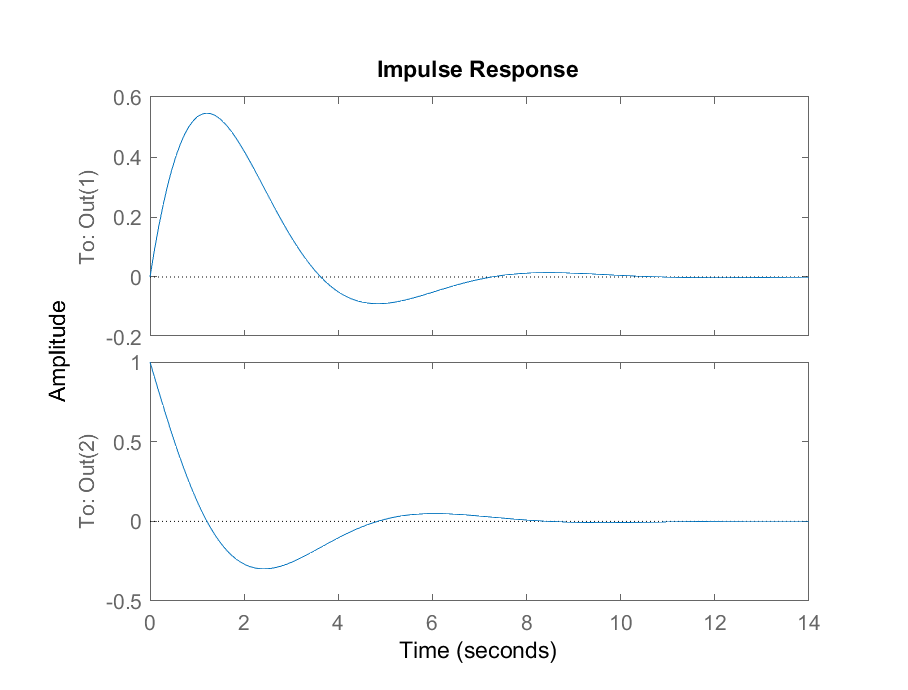
\includegraphics[width=0.7\textwidth]{impulse_response_msd.eps}
	\caption{Impulse response plot of the mass damper spring system.}
\end{figure}

Since we are considering the impulse responce of the system, we know that the input will be constant zero. Hence we will consider the system to be unforced for the time being. We will use the data to reconstruct the $A$ matrix of the system.

In the case of system identification we need that the matrix containing both $X_-$ and $U_-$ is full rank. Since our input data is constant zero we will not be able to identify the discrete time system matrices $A_d$ and $B_d$. However, due to our input being zero we are able to consider the system as if it had no input and hence we are able to identify the descrete time $A_d$ matrix. Note that for our state data to be compatible with the function from the toolbox we need to transpose is to be a wide matrix instead of a tall one.

\begin{lstlisting}
x = x';
[bool, A_d] = isInformIdentification(x)
\end{lstlisting}

Which will return that the data is indeed informative for system identification and gives us the following discrete time $A_d$ matrix.

\begin{equation*}
	\begin{bmatrix}
		 0.9959 &   0.0879 \\
		-0.0879 &   0.9080
	\end{bmatrix}
\end{equation*}

Now we need to verify that the continuous time counterpart of this descrete time $A_d$ matrix is indeed the same as our original system. For this we will use the function \mon{sysc = d2c(sysd)} provided by matlab to transform a discrete time system to a continuous time system. Note that we need to define a time step for our discrete time system, we can retreive the time step from the \mon{t} matrix returned by the impulse responce function.

\begin{lstlisting}
sys_d = ss(A_d, [], [], [], t(2));
A_c = d2c(sys_d).A
\end{lstlisting}

This will return the following continuous time $A_c$ matrix.

\begin{equation*}
	\begin{bmatrix}
		-0.0000 &   1.0000\\
		-1.0000 &  -1.0000
	\end{bmatrix}
\end{equation*}

As we can see our computed $A_c$ matrix is almost the same as the true $A$ matrix. The larges difference as computed by matlab between entries of the matrices is $0.3e-14$ which makes them the same up to machine precision.

\subsection{Step response}
We will now be considering the step responce of the system. We will pick our input to be constant $1$. Using this we will repeat the previous steps to see if we are able to accuratly recover both the $A$ and $B$ system matrices. We will generate the data using the built in Matlab function \mon{[y, t, x] = step(sys)}. 

\begin{lstlisting}
[~, t, x] = step(sys_c);
\end{lstlisting}

\begin{figure}[H]
	\centering
	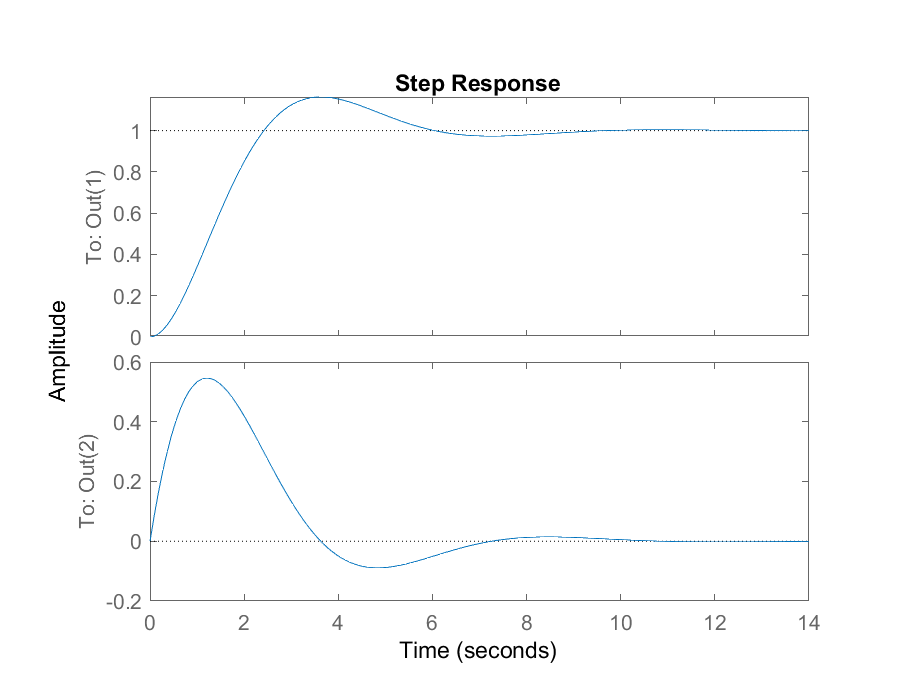
\includegraphics[width=0.7\textwidth]{step_response_msd.eps}
	\caption{Step response plot of the mass damper spring system.}
\end{figure}

Since our input data is non zero it might be the case that the matrix containing both $X_-$ and $U_-$ is full rank. Before we check if the data is informative for system identification we will prepare teh data to be used for the toolbox.

\begin{lstlisting}
x = x';
U = ones(1,size(x,2) - 1);
[bool, A_d, B_d] = isInformIdentification(x, U)
\end{lstlisting}

From this we can indeed see that the data is informative for system identification and that the discrete time system matrices are given as:

\begin{align*}
	A_d &= \begin{bmatrix} 0.9959 & 0.0879 \\ -0.0879 & 0.9080 \end{bmatrix} &
	B_d &= \begin{bmatrix} 0.0041 \\ 0.0879 \end{bmatrix} 
\end{align*}

We will once again convert these to a continuous time system using \mon{sysc = d2c(sysd)} with the time step as defined in the \mon{t} matrix returned by the step function.

\begin{lstlisting}
sys_d = ss(A_d, B_d, [], [], t(2));
A_c = d2c(sys_d).A
B_c = d2c(sys_d).B
\end{lstlisting}

Which will return the following continuous time system matrices.

\begin{align*}
A_d &= \begin{bmatrix} 0.0000 & 1.0000 \\ -1.0000 & -1.0000 \end{bmatrix} &
B_d &= \begin{bmatrix} 0.0000 \\ 1.0000 \end{bmatrix} 
\end{align*}

As we can see the computed continuous time system matrices are again the same as the true system up to machine presision.
\newpage
%\section{How to use the toolbox for linearising models}\newpage
%\section{Improving controller performance using H$_2$}\newpage


% ----------------------------- Discussion and conclusion
\section{Conclusion}
The aim of this project was to implement the methods discussed in the informativity framework from \cite{waarde2019data} and \cite{waarde2020noisy} for computation of system theoretic properties and controller directly from data into Matlab as well as providing documentation for each methods.

This is done by providing a look at how the methods were derived in the documentation as well as providing corresponding functions for each method. This was done for all the methods described in the previously mentioned papers. The documentation also provides examples for each of the methods as well as an example of how the functions can be used for system identification on continuous-time systems using the impulse and step response. 

All these methods are implemented and available at: \\
\url{http://github.com/JeroenLam/Matlab-Toolbox-for-Data-driven-Control}

% ----------------------------- Future work
\input{31FutureWork}
% ----------------------------- Limitations -------------------------

% ----------------------------- Acknowladgements --------------------
\section{Acknowledgements}
I would like to thank dr. Henk J. van Waarde for his time and help with coordinating the project.
% ----------------------------- References --------------------------
\section{Reference section title}
\printbibliography[heading=bibintoc,title={References}]
\todo{Fix S in dynamic measurement feedback}
% ----------------------------- Apendix ----------------------------- 


\end{document}



